\chapter{Baseline speech synthesis}

%This chapter explain how the project was carried out
%In this chapter of the document, the development process that has been followed in order to complete this project is explained.

%This chapter explains how the baselin was developed. The methodologies and technologies that were used during this project are also discussed.

\section{Baseline development}

The first stage of this project was to develop a baseline speech synthesizer. This model is used as a reference when comparing the results of the experiments explained in the evaluation chapter. The architecture is based on the work done by \cite{pascual2016deep} by using the Socrates Text-to-speech framework developed in the VEU research group at UPC, which is based on the Keras deep learning library. This is a RNN-LSTM based model, which, as mentioned in section \ref{sec:rnn-tts}, contains a duration model and an acoustic model which are trained independently.

\tikzstyle{layer} = [rectangle, draw, fill=blue!20, text centered, minimum width=19em, minimum height=2em]

\begin{figure}[h]
    \centering
    %\includegraphics[width=8cm]{figures/cat}
    \begin{tikzpicture}[auto]
        % duration model
        \node [minimum width=19em](dur) {\textbf {Duration model}};
        \node[layer, below of=dur, fill=gray!20] (input0) {\tiny Input (330)};
        \node[layer, below of=input0, fill=green!20] (lstm0) {\tiny LSTM (256)};
        \node[layer, below of=lstm0] (fc2) {\tiny (Output) Fully connected (1)};

        % acoustic
        \node[minimum width=19em, right=1em of dur] (aco) {\textbf{Acoustic model}};
        \node[layer, below of=aco, fill=gray!20] (input1) {\tiny Input (332)};
        \node[layer, below of=input1] (fc0) {\tiny Fully connected (256)};
        \node[layer, below of=fc0] (fc1) {\tiny Fully connected (256)};
        \node[layer, below of=fc1, fill=green!20] (lstm0) {\tiny LSTM (512)};
        \node[layer, below of=lstm0, fill=green!20] (lstm1) {\tiny LSTM (512)};
        \node[layer, below of=lstm1] (fc2) {\tiny (Output) Fully connected (43)};
    \end{tikzpicture}
    \caption{Baseline models.}
    \label{fig:lstm-tts}
\end{figure}

\begin{itemize}
    \item The duration model predicts the duration of a phoneme. This model takes a vector of linguistic features with information about the phoneme and its context and outputs a single value that is the log-compressed duration of the phoneme (this log-compression is explained in the data preparation section).
    \item The acoustic model predicts the excitation and spectral parameters of a frame of speech. The input of this system is the same vector of linguistic features, the normalized duration of the predicted value from the previous model and the relative position of the frame within the duration of the phoneme. The output of this model is also explained in the next section.
\end{itemize}

%The baseline architecture of the system was not developed from scratch but the preparation of the data used to train and test the system had to. In this chapter the data preparation and development of the systems is explained.

%The overall system, without going in depth in the system is the one shown in Figure \ref{fig:sys}, where a set of acoustic features are produced from the audio streams and another set of linguistic features are obtained from the transcriptions.

%In the following subsections we go in more detail into each of the shown modules from Figure \ref{fig:sys}. The explanations are not a special case of the baseline system but they are also relevant for the final system with the added expressiveness features from the other sections of this chapter.
%The following sections explain how the data that is used to train this architecture is obtained from our speech corpus.

\section{Data preparation}

%The developed speech synthesizer is an RNN-based architecture similar to the one presented in chapter 2. As mentioned in that section, the architecture from the baseline system is composed of two sections: a duration model and an acoustic model. It is important to note that this system does not produce the output waveform directly but instead it produces spectral and excitation coefficients like in SPSS based systems. This means that the speech database that we use will have to be processed in order to train the system.

The corpus that has been used for this project contains approximately 20 hours or audiobooks along with the transcripts. This corpus was originally produced for the Blizzard challenge \cite{blizzard} and is already segmented at the utterance level, removing the need to align the whole audio stream with the raw text data. The reason we chose this corpus is because of its richness in expressive content. Table \ref{tab:blizard} shows some information about the audio files that we get from it.

% table with audio information (Sampling, bit depth, channels, etc...)
\begin{table}[h]
    \centering
    \begin{tabular}{l|c}
        Metric & Value \\
        \hline
        Sampling rate ($Hz$) & 16000 \\
        Bit depth (bits) & 16 \\
        Channels & mono \\
        Length (seconds mean) & 7.23 \\
        Length (seconds std) & 4.52 \\
        Speakers & 1
    \end{tabular}
    \caption{Information about the Blizzard Challenge utterances.}
    \label{tab:blizard}
\end{table}

%Every speech waveform is decoded at a frame level by using a vocoder using a sliding window that advances 5 milliseconds between consecutive windows. The vocoder that we used for this project is Ahocoder, an Harmonics plus Noise Model that is described in detail at \cite{vocoder_ah}. In Figure \ref{fig:wav-prep} it is shown how each utterance is processed.

\section{Obtaining Acoustic features} \label{sec:aco-features}

As mentioned in section \ref{sec:rnn-tts}, this RNN based speech synthesizer is based on SPSS and as such it doesn't output the waveforms directly but the excitation and spectral parameters before they are reconstructed by a vocoder. The vocoder that we used is Ahocoder \cite{vocoder_ah}.

Every audio file is framed by means of a sliding window with a stride of 5 milliseconds. Ahocoder then processes each frame to produce a set of excitation and spectral parameters which are:

\begin{itemize}
    \item{Mel Frequency Cepstral Coefficients (MFCC) of order $p = 39$, which corresponds to $40$ coefficients. This represents the information from the speech formants.}
    \item{Pitch contour ($log(F_0)$). Unvoiced frames correspond to $F_0 = 0$. Ahocoder outputs a value of $-10^8$ when the frame is unvoiced.}
    \item{Maximum voiced frequency ($fv$), This value is 0 when a frame is unvoiced.}
    \item{Voiced/Unvoiced (UV) flag. This value indicates if a given frame of audio corresponds to a voiced or unvoiced sound and is obtained using the $log(F_0)$ output of Ahocoder.}
\end{itemize}

To perform this data extraction from the Blizzard corpus, the Python and Bash scripting languages were used to parallelize the whole process. The basic unit of work of this step is to spawn an Ahocoder process with the path of the file, and save the speech parameters that it generates to disk. Because this operation is single threaded, and because of the large amount of data that we had in the Blizzard Challenge dataset (20 hours of speech), this process was parallelized in order to fully utilize the computing resources of the server. This involved writing two scripts:

\begin{itemize}
    \item \textbf{split\_names.py} is a Python script that takes a list of files (All the filenames from the Blizzard corpus) and splits it into smaller chunks.
    \item \textbf{process\_ahocode.sh} is a Bash script that reads a list of files and processes each of them through Ahocode and saves the speech parameters to the disk.
\end{itemize}

The filenames of the corpus was split into 30 chunks (the server has 32 CPUs) using the \textbf{split\_names.py} script and each of the chunks was processed by \textbf{process\_ahocode.sh}. Using this method inspired by \cite{pascual2016deep} this whole data preparation process was accomplished in less than one hour fully utilizing the system resources.

\begin{comment}
\begin{figure}
    \centering
    \includegraphics[width=15cm]{figures/ahoload}
    \caption{Full utilization of system resources by Ahocoder. Memory and CPU usage are close to their limits.}
    \label{fig:aho-load}
\end{figure}
\end{comment}

\section{Acoustic feature normalization}

The data is not used as it is at the output of the Ahocoder directly. These acoustic predictors are normalized before they are used to train the acoustic model for a good behavior of the back-propagation algorithm, as discussed in \cite{pascual2016deep}.

The outputs of the Ahocoding process ($MFCC$, $log(f_0)$ and $f_v$) were normalized so that they were bound between a minimum and a maximum value range. This range is chosen to be ${0.01, 0.99}$. The normalization of the acoustic outputs is shown in equation \ref{eq:out-norm}

\begin{equation}
    \hat{y} = 0.01 + (0.99 - 0.01) \frac{y - y_{min}}{y_{max} - y_{min}}
    \label{eq:out-norm}
\end{equation}

This doesn't work for the $log(F_0)$ features however. Because Ahocoder outputs a value of $-10^8$ when a frame is not voiced, equation \eqref{eq:out-norm} would compress the values from the voiced frames too much. \cite{pascual2016deep} solves it by keeping the values from the voiced frames and interpolating the values in the unvoiced regions as shown in Equation \ref{eq:linear-f0}:

\begin{equation}
    log F_0^i = log F_0^p + (log F_0^n - log F_0^p) \cdot \frac{i-p}{n-p}
    \label{eq:linear-f0}
\end{equation}

Where $n$ is the next voiced frame's frame index, $F_0^n$ is the next voiced frame's first value, p is the previous voiced value's frame index, $F_0^p$ is the previous voiced value and $F_0^i$ is the $i$-th new interpolated value to be replaced in the original output of the Ahocoding process (Figure \ref{fig:f0-int} has an example of this interpolation). We can then use the UV flag to recover the original format after denormalization and reconstruct the waveform.

\begin{figure}[h]
    \centering
    \includegraphics[width=12cm]{figures/f0.png}
    \caption{$F_0$ contour interpolation}
    \label{fig:f0-int}
\end{figure}

%The audio transcriptions have to be segmented at phoneme level into the linguistic features of th system. This is done using both the audio and the transcriptions in a process called forced-alignment to obtain a prediction of the duration of each phoneme uttered in each sentence. This process and the linguistic features that come out of this process are explained in the following section:

These acoustic features are used to train the acoustic model of the system. The data is structured for training as a series of input-output vector pairs laid out in the following manner in the training data tables:

\begin{figure}[h]
\begin{lstlisting}
<linguistic features 1, duration 1> <acoustic features 1>
<linguistic features 1, duration 1> <acoustic features 2>
<linguistic features 1, duration 1> <acoustic features 3>
<linguistic features 2, duration 2> <acoustic features 4>
<linguistic features 2, duration 2> <acoustic features 5>
<linguistic features 2, duration 2> <acoustic features 6>
<linguistic features 2, duration 2> <acoustic features 7>
<linguistic features 3, duration 3> <acoustic features 8>
<linguistic features 3, duration 3> <acoustic features 9>
...
\end{lstlisting}
\caption{Training table used to train the acoustic model is stored in the server disk.}
\end{figure}

Which are the examples that are used to train the acoustic model. Some of the inputs are repeated depending on the duration of the phonemes (the linguistic features are explained in the next section). To create these tables, another python script \textbf{gen\_aco\_tables.py} was written for the project. This script reads a list of files corresponding to the single sentences from the Blizzard corpus and does the following:
\begin{enumerate}
    \item Reads the file of linguistic features (explained in the next section) containing both the phonetic segmentation and the phoneme durations.
    \item Reads the corresponding acoustic features from Ahocoder (obtained in the previous section) and writes a line containing: the vector of linguistic features, the log normalized duration of the phoneme, the relative position of the ahocoder window within the current phoneme, and the vector of acoustic features ($MFCC$, $log(f_0)$, $f_v$ and $UV$). This line in repeated for as many windows the phoneme lasts (modifying the relative duration value every line). At the end there might be a remainder duration error because the number of windows the phoneme lasts might not be an integer number. This remainder is carried to the next phoneme.
    \item Once all the data has been collected, the values are normalized and written to disk for use in Socrates.
\end{enumerate}

We execute this script for both the training data, the test data and the validation data. These can be done in parallel but it is not as critical.

\section{Obtaining linguistic features} \label{sec:ling-feat}

Each of the audio transcriptions was transformed into a lower level phonetic representation called Label that contains a set of both real and categorical descriptors with information about each phoneme and its context within a sentence. Table \ref{tab:lab-format} contains a description of the values that are included in this representation.

When a phoneme is converted into a Label, it has the following format:

%TODO formato del lab de ogmios
\begin{lstlisting}
p1^p2$-$p3$+$p4$=$p5~p6_p7/A:a1_a2_a3/B:b1-b2-b3~b4-b5&b6-b7#b8-b9$b10...
-b11!b12-b13;b14-b15|b16/C:c1+c2+c3/D:d1_d2/E:e1+e2~e3+e4&e5+e6#e7+e8...
/F:f1_f2/G:g1_g2/H:h1=h2~h3=h4|h4/I:i1_i2/J:j1+j2-j3
\end{lstlisting}

\singlespacing
\begin{longtable}[!htpb]{p{0.1\textwidth} p{0.9\textwidth}}
\toprule
\multicolumn{2}{c}{label format} \\
\cline{1-2}
Symbol    & Description \\
\midrule
p1      & phoneme identity before the previous phoneme \\
p2      & previous phoneme identity \\
p3*      & current phoneme identity \\
p4*		& next phoneme identity \\
p5*		& the phoneme after the next phoneme identity \\
p6*		& position of the current phoneme identity in the current syllable (forward) \\
p7*		& position of the current phoneme identity in the current syllable (backward) \\
\midrule
a1 & whether the previous syllable is stressed or not (0; not, 1: yes)\\
a2 & whether the previous syllable is accented or not (0; not, 1: yes)\\
%\caption*{\tablename{} \ref{table:lab_format} (continued)}\\
\toprule
a3 & number of phonemes in the previous syllable \\
b1* & whether the current syllable stressed or not (0: not, 1: yes)\\
b2* & whether the current syllable accented or not (0: not, 1: yes)\\
b3* & the number of phonemes in the current syllable\\
b4* & position of the current syllable in the current word (forward)\\
\caption*{\tablename{} \ref{table:lab_format} (continued)}\\
b5* & position of the current syllable in the current word (backward)\\
b6* & position of the current syllable in the current phrase(forward)\\
b7* & position of the current syllable in the current phrase(backward)\\
b8* & number of stressed syllables before the current syllable in the current phrase\\
b9* & number of stressed syllables after the current syllable in the current phrase\\
b10* & number of accented syllables before the current syllable in the current phrase\\
b11* & number of accented syllables after the current syllable in the current phrase\\
b12* & number of syllables from the previous stressed syllable to the current syllable\\
b13* & number of syllables from the current syllable to the next stressed syllable\\
b14* & number of syllables from the previous accented syllable to the current syllable\\
b15* & number of syllables from the current syllable to the next accented syllable\\
b16* & name of the vowel of the current syllable\\
\midrule
c1* & whether the next syllable stressed or not (0: not, 1:yes) \\
c2* & whether the next syllable accented or not (0: not, 1:yes) \\
c3* & the number of phonemes in the next syllable \\
\midrule
d1 & gpos (guess part-of-speech) of the previous word \\
d2 & number of syllables in the previous word \\
\midrule
e1* & gpos (guess part-of-speech) of the current word \\
e2* & number of syllables in the current word \\
e3* & position of current word in the current phrase (forward) \\
e4* & position of current word in the current phrase (backward) \\
e5* & number of content words before the current word in the current phrase \\
e6* & number of content words after the current word in the current phrase \\
e7* & number of words from the previous content word to the current word \\
e8* & number of words from the current word to the next content word \\
\midrule
f1* & gpos (guess part-of-speech) of the next word \\
f2 & number of syllables in the previous word \\
\midrule
g1 & number of syllables in the previous phrase \\
g2 & number of words in the previous phrase \\
\midrule
h1* & number of syllables in the current phrase \\
%\caption*{\tablename{} \ref{table:lab_format} (continued)}\\
\toprule
h2* & number of words in the current phrase \\
h3* & position of the current phrase in utterance (forward) \\
h4* & position of the current phrase in utterance (backward) \\
h5* & Phrase modality (question, exclamation, etc.)\\
\midrule
i1* & number of syllables in the next phrase \\
i2 & number of words in the previous phrase \\
\midrule
j1* & number of syllables in this utterance \\
j2* & number of words in this utterance \\
j3* & number of phrases in this utterance \\
\bottomrule
\caption{\label{table:lab_format}Label format. The symbols tagged with an asterisk reference the future context of the phoneme.}\\
\label{tab:lab-format}
\end{longtable}
\doublespacing


A full example of this conversion is shown in Figure \ref{fig:sentence-lab}:

\begin{figure}[h]
\begin{lstlisting}[basicstyle=\tiny,frame=single]
pau^D-i+O:=t~2_1/A:0_0_2/B:0-0-2~1-1&1-10#0-0$0-2!0-0;3-4|i/C:0+0+1/D:NN_2/E:DT+1~1+5&0+3#0+1/F:...
D^i-O:+t=@~1_1/A:0_0_2/B:0-0-1~1-6&2-9#0-0$0-2!0-0;4-3|O:/C:0+0+2/D:DT_1/E:NN+6~2+4&0+3#1+1/F:IN...
i^O:-t+@=b~1_2/A:0_0_1/B:0-0-2~2-5&3-8#0-0$0-2!0-0;5-2|@/C:0+0+2/D:DT_1/E:NN+6~2+4&0+3#1+1/F:IN_...
O:^t-@+b=aI~2_1/A:0_0_1/B:0-0-2~2-5&3-8#0-0$0-2!0-0;5-2|@/C:0+0+2/D:DT_1/E:NN+6~2+4&0+3#1+1/F:IN...
t^@-b+aI=Q~1_2/A:0_0_2/B:0-0-2~3-4&4-7#0-0$0-2!0-0;6-1|aI/C:0+1+1/D:DT_1/E:NN+6~2+4&0+3#1+1/F:IN...
@^b-aI+Q=g~2_1/A:0_0_2/B:0-0-2~3-4&4-7#0-0$0-2!0-0;6-1|aI/C:0+1+1/D:DT_1/E:NN+6~2+4&0+3#1+1/F:IN...
b^aI-Q+g=r~1_1/A:0_0_2/B:0-1-1~4-3&5-6#0-0$0-1!0-0;7-5|Q/C:0+0+3/D:DT_1/E:NN+6~2+4&0+3#1+1/F:IN_...
aI^Q-g+r=@~1_3/A:0_1_1/B:0-0-3~5-2&6-5#0-0$1-1!0-0;1-4|@/C:0+0+2/D:DT_1/E:NN+6~2+4&0+3#1+1/F:IN_...
Q^g-r+@=f~2_2/A:0_1_1/B:0-0-3~5-2&6-5#0-0$1-1!0-0;1-4|@/C:0+0+2/D:DT_1/E:NN+6~2+4&0+3#1+1/F:IN_1...
g^r-@+f=i~3_1/A:0_1_1/B:0-0-3~5-2&6-5#0-0$1-1!0-0;1-4|@/C:0+0+2/D:DT_1/E:NN+6~2+4&0+3#1+1/F:IN_1...
r^@-f+i=@~1_2/A:0_0_3/B:0-0-2~6-1&7-4#0-0$1-1!0-0;2-3|i/C:0+0+2/D:DT_1/E:NN+6~2+4&0+3#1+1/F:IN_1...
@^f-i+@=v~2_1/A:0_0_3/B:0-0-2~6-1&7-4#0-0$1-1!0-0;2-3|i/C:0+0+2/D:DT_1/E:NN+6~2+4&0+3#1+1/F:IN_1...
f^i-@+v=@~1_2/A:0_0_2/B:0-0-2~1-1&8-3#0-0$1-1!0-0;3-2|@/C:0+0+1/D:NN_6/E:IN+1~3+3&1+2#1+2/F:DT_1...
i^@-v+@=h~2_1/A:0_0_2/B:0-0-2~1-1&8-3#0-0$1-1!0-0;3-2|@/C:0+0+1/D:NN_6/E:IN+1~3+3&1+2#1+2/F:DT_1...
@^v-@+h=O:~1_1/A:0_0_2/B:0-0-1~1-1&9-2#0-0$1-1!0-0;4-1|@/C:0+1+3/D:IN_1/E:DT+1~4+2&2+1#1+1/F:NN_1...
v^@-h+O:=s~1_3/A:0_0_1/B:0-1-3~1-1&10-1#0-0$1-0!0-0;5-0|O:/C:0+0+0/D:DT_1/E:NN+1~5+1&2+1#2+0/F:SI...
@^h-O:+s=pau~2_2/A:0_0_1/B:0-1-3~1-1&10-1#0-0$1-0!0-0;5-0|O:/C:0+0+0/D:DT_1/E:NN+1~5+1&2+1#2+0/F:...
h^O:-s+pau=_~3_1/A:0_0_1/B:0-1-3~1-1&10-1#0-0$1-0!0-0;5-0|O:/C:0+0+0/D:DT_1/E:NN+1~5+1&2+1#2+0/F:...
O:^s-pau+_=_~1_1/A:0_1_3/B:0-0-1~1-1&0-11#0-0$0-2!0-0;1-0|_/C:0+0+0/D:NN_1/E:SIL+1~0+6&0+3#1+0/F:...
\end{lstlisting}
    \caption{Truncated label representation of the phrase "the autobiography of a horse."}
    \label{fig:sentence-lab}
\end{figure}

%To convert the sentences to these Label representations, along with a prediction of the duration of each phoneme so we can use them as examples to train the synthesizer models, the Ogmios framework \cite{bonafonte2006ogmios} was used during the development of this project. In this program, a series of modules are combined in order to perform the task of phoneme segmntation and duration prediction. Figure \ref{fig:ogmios-pipeline} shows the Ogmios modules:

To obtain the Labels of the Blizzard corpus, first the sentences were phonetically segmented. This process was done using the Ramses and Ogmios \cite{bonafonte2006ogmios} software. The whole process was mostly automated following a guide:

\begin{enumerate}
    \item The text files are converted to their phonetic representation. Speech parameters are also computed from the audio files from where a codebook is created and quantized.
    \item The next step estimates a semi-continuous HMM, where only the GMM parameters are quantized, for every phonem using the speech parameters. Using these HMM models and the phonetic transcriptions, a force alignment is performed to find the transitions of the phonemes and the internal pauses and silences in the sentences using the Viterbi algorithm.
    \item Next it creates a diphone transcription \cite{marino1997demiphone} of the sentences and estimates an HMM of them.
    \item Finally, a force alignment is performed again to obtain the diphone transitions in order to compute the duration of each phoneme.
    \item A script is called to convert the outputs from the Ogmios program to the Label representation with the phoneme durations.
\end{enumerate}

\begin{comment}
This label conversion is carried out with the aid of the Ramses and Ogmios software \cite{bonafonte2006ogmios}. This programs offers a collection of speech processing modules that are combined to perform a task. For the case of this project, 

%it was used to obtain this label representation and to predict the duration of each of the phonemes in the sentences from the Blizzard corpus. Figure \ref{fig:ogmios-pipeline} shows the steps that it takes to obtain this information:

\tikzstyle{block} = [rectangle, draw, fill=blue!20, text width=6em, text centered, rounded corners, minimum height=4em]
\tikzstyle{red-block} = [ellipse, draw, fill=blue!20, text width=6em, text centered, rounded corners, minimum height=4em]
\tikzstyle{line} = [draw, -latex']

\begin{figure}[h]
    \centering
    \begin{tikzpicture}[node distance = 3cm, auto]
        \node[block] (bl0) {\tiny (1) Text normalization};
        \node[block, right of=bl0] (bl1) {\tiny (2) Phonetic transcription};
        \node[block, right of=bl1] (bl2) {\tiny (3) Context dependant HMMs};
        \node[block, right of=bl2] (bl3) {\tiny (4) Force alignment};
        \node[block, right of=bl3] (bl4) {\tiny Label format};
        \path[line] (bl0) -- (bl1);
        \path[line] (bl1) -- (bl2);
        \path[line] (bl2) -- (bl3);
        \path[line] (bl3) -- (bl4);
    \end{tikzpicture}

    \caption{Ogmios modules used to predict phoneme duration.}
    \label{fig:ogmios-pipeline}
\end{figure}

\begin{enumerate}
    \item The text normalization module converts numeric values, dates, etc to its corresponding text form.
    \item The phonetic transcription module provides the pronunciation of the words.
    \item The HMM module estimates a left-to-right HMM model for each of the phonemes (Figure \ref{fig:hmm}) using the speech spectral parameters.
    %\item For each of the sentences it chains their phoneme HMMs and computes the most probable sequence of states to predict the duration of each phoneme using the V algorithm.
    \item Given the phonemes of a sentence, it chains the HMM models and the most probable sequence of states is calculates using the Viterbi algorithm. With this information it can calculate the duration of each phoneme by finding the HMM model transitions.
    \item The phonetic transcriptions along with the duration predictions are converts to the label format from table \ref{tab:lab-format}.
\end{enumerate}
\end{comment}

\section{Linguistic features normalization}

The linguistic features, also had to be normalized prior to training. As seen previously, the label format contains both categorical features and real features. The categorical information was encoded so that all categories are orthogonal to each other by using a one-hot encoding. As a small example of a one-hot encoding, consider the three categories $\{A, B, C\}$. The  one-hot encoding for the three categories is $\{(1,0,0), (0,1,0), (0,0,1)\}$.

The real features from the acoustic features are normalized so that the mean equals zero and the standard deviation equals one for each of them. This operation is called z-norm and it is shown in \ref{eq:znorm}.

\begin{equation}
    z = \frac{x - \mu}{\sigma}
    \label{eq:znorm}
\end{equation}

The predicted duration of each phoneme was log-compressed to avoid having a long-tailed distribution that can distort the training of the model when using the Mean Square Error (MSE) minimization as discussed in \cite{pascual2016deep}. Figure \ref{fig:hist-d} contains the histogram of the raw predicted durations and the histogram after the log-compression operation. This operation was performed by simply taking the natural logarithm of the stored phoneme durations:

\begin{equation}
    \hat{d} = log(d)
\end{equation}
%Instead of predicting the duration in milliseconds produced by Ogmios, we take the logarithm to avoid having a long tailed distribution that distorts the training using the Mean Square Error (MSE) minimization as discussed in \cite{pascual2016deep}. Figure \ref{fig:hist-d} contains the histogram of these values before and after the log operation.

\begin{figure}[h]
    \centering
    \includegraphics[width=14cm]{figures/dur}
    \caption{Histogram of the phoneme duration predictions by Ogmios.}
    \label{fig:hist-d}
\end{figure}

Once we have obtained the linguistic features, we discard of those who reference the past and only keep the ones tagged with an asterisk ($*$) in Table \ref{tab:lab-format}. This is because the models are based on LSTM-RNN which are known to be good at modeling long term dependencies from the past\cite{hochreiter1997long}.

\section{Training of the baseline}

As mentioned before, the system is developed within the Socrates Test-to-speech framework. In the version that was used, this program allows us to define the full architecture in a plain-text configuration file. In this file we specify the number of layers, inputs parameters, the paths where the training, test and validation data are stored in the disk, and the path where to store the intermediate files that the framework generates during training (network weights, loss curves and cached information). An example of configuration file is shown in Figure \ref{fig:soc-conf}.

\begin{figure}[h]
    \begin{lstlisting}[basicstyle=\small,frame=single]
[[tts_core]]                                       
name="labdecode_core"

[[tts_core]]                                       
name="dur_rnn_core"                                
topology="baseline/dur_rnn_core-eng.cfg"           
dur_stats="model/73/dur/dur.stats.train"            
train_table="../tables/duration/baseline/train.dur"
test_table="../tables/duration/baseline/test.dur"  
valid_table="../tables/duration/baseline/valid.dur"
loss_path="baseline/loss_curves/"                  
tables_cache_path="baseline/tables_cache"          
                                                   
[[tts_core]]                                       
name="dur2aco_norm_core"                           
dur_stats="model/73/dur/dur.stats.train"

[[tts_core]]
name="aco_rnn_core"
dur_stats="model/73/aco/dur.stats.train"
aco_stats="model/73/aco/aco.stats.train"
train_table="../tables/acoustic/baseline/train.aco"
test_table="../tables/acoustic/baseline/test.aco"
valid_table="../tables/acoustic/baseline/valid.aco"
topology="baseline/aco_rnn_core-eng.cfg"
tables_cache_path="baseline/tables_cache"
loss_path="baseline/loss_curves/"

[[tts_core]]
name="ahodecode_core
    \end{lstlisting}
    \caption{Configuration example for the baseline system. Some options have been omitted.}
    \label{fig:soc-conf}
\end{figure}

In this example, we specify that this model is composed of five modules, called cores within the framework. Each of these cores perform the following actions

\begin{enumerate}
    \item \textbf{labdecode\_core} decodes the label format from Section \ref{sec:ling-feat} and converts it to the input that the model expects (converts the categories to one-hot and normalizes the numeric values)
    \item \textbf{dur\_rnn\_core} predicts the duration of the phoneme that was provided from the previous core.
    \item \textbf{dur2aco\_norm\_core} denormalizes the predicted duration and generates the input features that are feed to the acoustic model. It also adds the durations and relative durations as mentioned at the beginning of this chapter.
    \item \textbf{aco\_rnn\_core} predicts the acoustic features explained in Section \ref{sec:aco-features}.
    \item \textbf{ahodecode\_core} takes the output from the previous core, formats the data to be input to the Ahodecoder, and produces a WAVE file containing the synthesized speech.
    %\item \textbf{ahodecode\_core} takes the output from the previous core, formats the data to be input to the Ahodecoder, and produces a WAVE file containing the synthesized speech.
\end{enumerate}

The configuration file also has access to the "stats" of the features that contain the minimum and maximum values so that the compression from \ref{eq:out-norm} can be undone.
%The two models: duration and acoustic, also have access to information about the minimum and maximum values of the input and output features so that the min-max compression can be undone.

As mentioned previously, the Blizzard Challenge corpus contains roughly twenty hours of speech data. Due to complications loading the data into memory using the framework, we had to cut the total amount down to 30\% to train the acoustic model. Newer releases of this framework deal with this problem so it can handle the full corpus data.

This chapter has covered the baseline architecture, data preparation and training. The next step of the project was to add expressive features to the system. The following chapter focuses on this.

\chapter{Expressive speech synthesizer}

%TODO
Once we had the system up and running it was time to introduce the modifications that would allow for expressive speech to be modeled by the system. The way this is done in this project is by introducing a new set of features as inputs to the system (both the duration and acoustic model). These are known as the embeddings that encapsulate the information about the way a given sentence is supposed to be synthesized like, given its semantic content, and they are used alongside the linguistic features from the baseline system. In this section we describe the process of obtaining these new features. Other than these new inputs, the developed system shares the same architecture from the baseline system.

\section{Sentiment analysis \& embedding extraction task} \label{sec:sa}

\tikzstyle{layer} = [rectangle, draw, fill=blue!20, text centered, minimum width=19em, minimum height=2em]

\begin{comment}
\begin{figure}[h]
    \centering
    %\includegraphics[width=8cm]{figures/cat}
    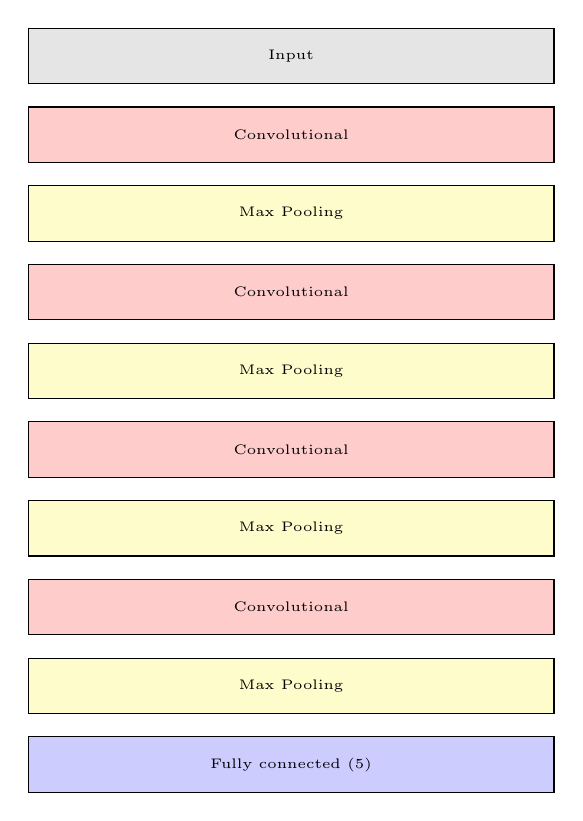
\begin{tikzpicture}[auto]
        % duration model
        \node[layer, fill=gray!20] (input0) {\tiny Input};
        \node[layer, below of=input0, fill=red!20] (conv0) {\tiny Convolutional};
        \node[layer, below of=conv0, fill=yellow!20] (conv0) {\tiny Max Pooling};
        \node[layer, below of=conv0, fill=red!20] (conv0) {\tiny Convolutional};
        \node[layer, below of=conv0, fill=yellow!20] (conv0) {\tiny Max Pooling};
        \node[layer, below of=conv0, fill=red!20] (conv0) {\tiny Convolutional};
        \node[layer, below of=conv0, fill=yellow!20] (conv0) {\tiny Max Pooling};
        \node[layer, below of=conv0, fill=red!20] (conv0) {\tiny Convolutional};
        \node[layer, below of=conv0, fill=yellow!20] (conv0) {\tiny Max Pooling};
        \node[layer, below of=conv0] (conv0) {\tiny Fully connected (5)};
    \end{tikzpicture}
    \caption{Baseline models.}
    \label{fig:lstm-tts}
\end{figure}
\end{comment}

Once the baseline system was developed, the additions to the initial system were developed. These involve obtaining the expressive paragraph embeddings that would allow for the modeling of the expressiveness of the speech signal. We used sentiment analysis to capture the expressive information of the Blizzard Challenge dataset that was used in the baseline system. Because the sentences on this dataset are not made for sentiment analysis tasks, they lack the information to train a text classification system. To perform this text classification task, we used the Stanford sentiment treebank dataset \cite{socher2013recursive}, which contains a list of movie reviews. An example of a tagged sentence from this dataset is shown in figure \ref{fig:tree}.

\begin{figure}[h]
    \begin{lstlisting}[basicstyle=\small,frame=single]
(2 (3 (3 Effective) (2 but)) (1 (1 too-tepid) (2 biopic)))

Tag Sentence
2   Effective but too-tepid biopic
2   Effective but
3   Effective
2   but
1   too-tepid biopic
1   too-tepid
2   biopic
    \end{lstlisting}
    \label{fig:tree}
    \caption{Example of sentence tree corresponding to the sentence "Effective but too-tepid biopic"}
\end{figure}

Each of the nodes on the tree is tagged in a scale from 0 to 4, 0 meaning very negative and 4 being a very positive text. Each sub-sentence was tagged down to the single words of the sentence. We used this dataset to train a CNN-based classifier similar to \cite{DBLP:journals/corr/Kim14f}. This architecture is shown in Figure \ref{fig:cnn-sa}.

\begin{figure}[h]
    \centering
    \includegraphics[width=15cm]{figures/cnn}
    \label{fig:cnn-sa}
    \caption{Text classification architecture. The figure is originally from \cite{DBLP:journals/corr/Kim14f}}
\end{figure}

%The following list explains the different layers of the architecture:

\begin{itemize}
    \item The first layer is an embedding layer. Each word is transformed into a low dimensional (300) representation. This step converts a sentence into a signal suitable for the next convolutional layer. The embedding layer consists of a (N+1)*300 matrix where N is the size of the vocabulary and the $n$-th vector column corresponds to the embedding of the $n$-th word in the vocabulary. An extra column is used for words that are not from the vocabulary and contains a random value. This architecture in particular has two-channel inputs, one with trainable embeddings, and the other with fixed ones. Both embedding matrices are initialized to the Glove embeddings \cite{pennington2014glove}.
    \item A convolutional layer with filters of sizes 3, 4 and 5 with 100 feature maps each. 
    \item A max-over-time pooling operation \cite{collobert2011natural}, where we select the maximum value from each of the feature maps.
    \item A Fully connected layer with softmax activations that give the output of the classification task. This layer is regularized using the dropout method with dropout probability of $0.5$ \cite{srivastava2014dropout} and the weights of this network are constrained using l2 regularization.
\end{itemize}

We choose the max-over-time pooling layer activations to obtain the additional inputs that added to the baseline synthesizer model. There is an issue with using the Stanford treebank dataset to train this system. Because the dataset is based on movie reviews, the text domain doesn't belong to the same from the Blizzard challenge data, which is the one we use to train the synthesizer models. Therefore, the sentiment analysis network has to be adapted. The following section explains the methodology that was followed in order to attempt to achieve this task.

\section{Network domain adaptation}

To perform the domain adaptation, we do the same classification task on a different architecture using the Blizzard challenge data. This network makes the prediction with the audio files as inputs. As explained before, this dataset is not prepared for text classification therefore they lack the class tags needed. We obtain these by using the network from the previous section after it has been trained using the Stanford sentiment treebank dataset. In \cite{aytar2016soundnet} they train a waveform classifier using unlabeled audio files and a pre-trained network to obtain them from the video frames. We perform the same task using audio and text data instead.

This task is performed in two steps:

\begin{enumerate}
    \item We train the audio based network by using the text network to obtain the labels. Because the labels that we obtain for the Blizzard sentences are probabilities, we optimize the network using KL-divergence using standard back-propagation \cite{aytar2016soundnet}.
    \item After a fixed number of iterations, we fine tune \cite{yosinski2014transferable} the text network by using labels obtained from the audio network. At this point, the two networks take turns to perform a back-propagation pass. Because the state of the weight of each network is constantly changing, we intend to leak information about the audio files into the text network.
\end{enumerate}

\section{Training embeddings extraction and expressive synthesis}

\subsection*{Sentiment analysis task}

In order to train the embedding extraction, the Keras deep learning framework was used to define the two networks. First, the data had to be processed in order to train the system. As shown in Figure \ref{fig:tree}, the sentences in the Stanford sentiment treebank are provided by a tree representation. Each of these trees were traversed in order to collect all the sentences and sub-sentences of the dataset. Figure \ref{fig:sent-histo} shows the distribution of sentence lengths:

% table with audio information (Sampling, bit depth, channels, etc...)
\begin{figure}[h]
    \centering
    \includegraphics[width=10cm]{figures/sa-histo}
    \caption{Distribution of sentence lengths in the Stanford sentiment treebank dataset.}
    \label{fig:sent-histo}
\end{figure}

To train this sentiment analysis task, we use all the sentences from the training dataset that are $\ge 3$ in length (words). The test data however, only contains the root nodes of the sentences like they do in \cite{DBLP:journals/corr/Kim14f} and in the original paper from the dataset.

\subsection*{Domain adaptation task}

\begin{table}[h]
    \centering
    \begin{tabular}{l|c|c|c|c|c|c|c|c|c}
                     & conv & pool & conv & pool & conv & pool & conv & conv & conv \\
        \hline
        Feature maps & 32    & 32   & 64   & 64   & 128  & 128  & 256 & 512  & 5 \\
        Filter size  & 64    & 8    & 32   & 8    & 16   & 8    & 8   & 4    & 5 \\
        Stride       & 2     & 2    & 2    & 2    & 4    & 2    & 4   & 1    & 1 \\
    \end{tabular}
    \caption{CNN used to process the Blizzard waveforms.}
    \label{tab:sent-cnn}
\end{table}

%TODO
Once the sentiment analysis task is done, the same network has to be adapter for the aforementioned reasons. To perform this task, we define a CNN from Table \ref{tab:sent-cnn}. The reason for choosing a CNN architecture as opposed to a different one such a DNN is because of the high dimensionality of the input. As aforementioned, this network takes whole waveforms from the Blizzard corpus. Convolutional layers have less trainable parameters since the number only depends on the size of the filters and the number of feature maps. This network also contains pooling layers which reduce the dimensionality of the input \cite{scherer2010evaluation} and PReLU activations \cite{xu2015empirical} which are activations with trainable parameters. We then use the following methodology:

\begin{enumerate}
    \item The audio network is trained using the Blizzard challenge WAVE files. The label of a file is obtained by using the sentiment analysis network with the transcript. Perform a fixed number of back propagation passes to initialize the weights of the network. From this point, the networks will take turns in performing back-propagation steps.
    \item We perform a back-propagation in the text network using a batch of sentences from the Blizzard corpus. The labels are obtained like in step 1 using audio network to obtain the labels.
    \item We perform a back-propagation in the audio network using a batch of wave files from the Blizzard corpus. Again, use the text network to obtain the labels.
    \item repeat step 2 for  a fixed number of iterations.
\end{enumerate}

\section{Training the expressive speech synthesizer}

Once the expressive embeddings are extracted for every sentence in the Blizzard Challenge corpus, we include the new inputs to both the duration and the acoustic model from the baseline system. This is specified in a new Socrates configuration file. Every linguistic feature vector that is input to the system includes the additional features that correspond to the full sentence the given phonemes belong to. After that, the process of training the models is the same that was followed in the baseline system.

One last processing step is to normalize the embeddings by compressing them between the $[0, 1]$ range.

The next chapter shows the evaluation results of the project.
